% Created 2021-03-16 Tue 21:36
% Intended LaTeX compiler: pdflatex
\documentclass[a4paper]{article}
\usepackage[utf8]{inputenc}
\usepackage[T1]{fontenc}
\usepackage{graphicx}
\usepackage{grffile}
\usepackage{longtable}
\usepackage{wrapfig}
\usepackage{rotating}
\usepackage[normalem]{ulem}
\usepackage{amsmath}
\usepackage{textcomp}
\usepackage{amssymb}
\usepackage{capt-of}
\usepackage{hyperref}
\usepackage{minted}
\usepackage[margin=1in]{geometry}
\usepackage{minted}
\usepackage{multicol}
\bibliographystyle{plain}
\RecustomVerbatimEnvironment{Verbatim}{BVerbatim}{}
\renewcommand{\figurename}{Listing}
\newenvironment{Figure}
  {\par\medskip\noindent\minipage{\linewidth}}
  {\endminipage\par\medskip}


\author{Scott Mora - 201816428}
\date{}
\title{TinyIdris Program Synthesis\\\medskip
\large Marking Scheme: Experimentation}
\hypersetup{
 pdfauthor={Scott Mora - 201816428},
 pdftitle={TinyIdris Program Synthesis},
 pdfkeywords={},
 pdfsubject={},
 pdfcreator={Emacs 27.1 (Org mode 9.3)}, 
 pdflang={English}}
\begin{document}

\maketitle
\begin{center}
\vspace{15mm}
Submitted for the Degree of B.Sc. in Computer Science. \\
\vspace{15mm}
Except where explicitly stated all the work in this report, including appendices, is my own and was carried out during my final year. It has not been submitted for assessment in any other context. 
 \end{center}
\clearpage
\tableofcontents
\clearpage

\section{Introduction}
\label{sec:orgf1aad56}

Programming often involves implementing low level details that can become
repetitive and tedious. The goal of program synthesis is to automate as much of this as
possible, speeding up the process of software development and reducing
bugs that can be introduced through programmer error. There have been
attempts to synthesise programs from many different communities,
the approach considered here uses the type system to guide the synthesis
tool towards a solution by reducing the number of terms enumerated.
This approach targets a common pattern seen in functional languages,
recursion via pattern matching. Dependently typed programming languages, 
though not confined to being functional languages, are typically 
structured in this functional way, and allow a greater amount of 
information to be encoded within the types of programs. 

This style of programming has multiple benefits. By encoding more 
information within types it allows the type checker to pick up on 
potential bugs that otherwise may not be caught until run-time, it also 
allows certain impossible states to be us-representable within programs,
ensuring the correctness of programs by construction and limiting the use of fatal 
exceptions. Typically functional programs encourage more code reuse,
and functional definitions can be considerably shorter than their 
imperative counterparts, which can result in shorter, more readable code.

To see how this can impact program synthesis, we look at an example, 
and why type information increases our chances of success. 
We define the \texttt{List} data type, and aim to synthesise a definition for
the function `map' which. When given a function as a parameter, and a 
list, map applies the function to each element of the list, a commonly 
used pattern in functional programming. The list argument has been
pattern matched on, and the holes to be synthesised have been added,
denoted by \texttt{?name}.

\begin{center}
\begin{minted}[obeytabs=true,tabsize=2]{idris}
data List : Type -> Type where
  Nil  : List a
  (::) : {a : Type} -> a -> List a -> List a

map : (f : a -> b) -> (xs : List a) -> List b 
map f [] = ?map_rhs_1
map f (x :: xs) = ?map_rhs_1
\end{minted}
\end{center}

Filling in the first hole is straightforward, since the expected output 
is the \texttt{Nil} constructor. The second, however, is more interesting.
There are now multiple outputs that would satisfy the type checker. 
The desired output applies \texttt{f} to \texttt{x} and concatenates the result to the
recursive call using the \texttt{(::)} constructor. However, inserting the term
\texttt{[]} into the hole would also satisfy the type checker, indeed,
with previous systems implemented, this is exactly the synthesised 
value.

By providing the type checker with more information we are able to 
eliminate possible incorrect answers, reducing the number of incorrect 
answers returned, and increasing the speed by reducing the number of 
branches to be checked. By allowing types to depend on terms we are 
able to do this, as the following example displays.

\begin{center}
\begin{minted}[obeytabs=true,tabsize=2]{idris}
data Vector : Nat -> Type -> Type where
  Nil  : Vector 0 a
  (::) : {a : Type} -> a -> Vector n a -> Vector (1 + n) a

map : (f : a -> b) -> Vector n a -> Vector n b
map f [] = []
map f (x :: y) = f x :: map f y
\end{minted}
\end{center}

Vector describes a family of types, where `Lists' are indexed
by their length. The first hole remains unchanged, since there is 
only one term satisfying \texttt{Vector 0 b}, namely, \texttt{Nil}.
In the (::) case however, the empty vector is no longer valid,
since the type \texttt{Vector 0 b} \(\neq\) \texttt{Vector (1 + n) b},
allowing us to find the correct term. 

TinyIdris is a small dependently typed programming language.
Users interact with the TinyIdris system by loading their source files
into the TinyIdris Repl (Read Eval Print Loop). This paper will outline 
an approach to extend TinyIdris with program synthesis functionality via
commands in the repl.

\clearpage

\section{The TinyIdris System}
\label{sec:org2a24981}

\begin{center}
\begin{figure}[htbp]
\centering
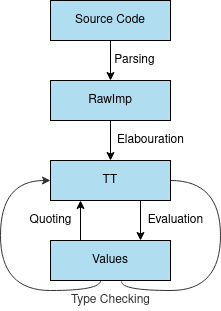
\includegraphics[scale=0.60]{./Resource/main.png}
\caption{TinyIdris processing order}
\end{figure}
\end{center}

TinyIdris is a dependently typed programming language with limited support
for implicit arguments. The language is a scaled down version of the 
Idris2 programming language, developed for teaching the implementation
of programming languages. The language is not compiled, instead, it comes
in the form of an executable program, which accepts the name of a 
Tiny Idris '.tidr' source file to be processed by the system.
The source code is converted into the internal representation of
the language, type checked, and each definition is stored in
memory. After the file has been processed, a read eval print loop, or 
repl is presented, which accepts expressions from the language,
evaluates them, and prints out the result.

\begin{center}
\begin{figure}[htbp]
\centering
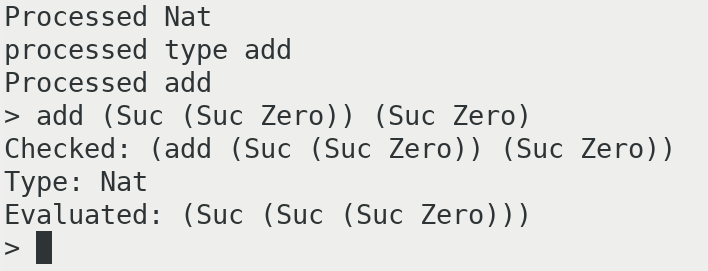
\includegraphics[scale=0.35]{./Resource/addEval.png}
\caption{Evaluating 2 + 1}
\end{figure}
\end{center}

\subsection{The Source code}
\label{sec:org85decd2}
Tiny Idris source code files consist of three top level global 
declarations, Data Types, Type Signatures, and Function Definitions,
each of which has their own local scope. 

\begin{center}
\begin{minted}[obeytabs=true,tabsize=2]{idris}
data Nat : Type where
 Zero : Nat
 Suc  : Nat -> Nat

add : Nat -> Nat -> Nat
add Zero m = m
add (Suc n) m = Suc (add n m) 

multiply : Nat -> Nat -> Nat
\end{minted}
\end{center}

\subsubsection{Type Signatures}
\label{sec:org6cd40f9}
Type signatures outline the shape of the data that is being transformed.
Written \texttt{f:a\textsubscript{1} ... a\textsubscript{n} -> r}, where \texttt{f} is the name, \texttt{a\textsubscript{1} ...  a\textsubscript{n}} are
the parameters, and \texttt{r} is the return type, read "f has type, a\textsubscript{1} 
to \ldots{} a\textsubscript{n} to r. Types in dependently typed languages are first class,
meaning it may take in any term, not just types, this includes function
types, and can be taken further, including types that contain data constructors and case expressions, however this is outwith the scope of
this paper. There can be 0 or more arguments,
however there must be exactly one return type, if multiple values are 
returned this is done so by constructing a tuple,
\texttt{f : a\textsubscript{1} ... a\textsubscript{n} -> (r, r', r'')}. Type signatures are present in both
of the following constructs.

\subsubsection{Data Types}
\label{sec:orga233947}
Data type declarations define a type, and describe how to construct it.
They consist of a type signature for the type being 
defined, known as a type declaration, and a set of data declarations, 
which are type signatures for each of the constructors.
The data type declaration begins with the keyword \texttt{data} and is followed by 
the type declaration. The data constructors are defined in the \texttt{where} 
clause that follows the type declaration. A type may have zero or more
data constructors. 

This style encourages inductive definitions, where the base case is 
defined, from which the other cases are built up, as seen in the \texttt{List},
\texttt{Vec}, and \texttt{Nat} examples. Defining Booleans however, we see that this
need not always be the case. 

\begin{center}
\begin{minted}[obeytabs=true,tabsize=2]{idris}
data Bool : Type where
  True : Bool
  False : Bool

data Nat : Type where
  Zero : Nat
  Suc  : Nat -> Nat

two : Nat
two = Suc (Suc Zero)
\end{minted}
\end{center}

Constructing the number two, we call the Successor constructor twice, first with the argument Zero,
and again with the result.

\subsubsection{Function Definitions}
\label{sec:org19c74b8}
The above example is a function definition, which has no arguments,
and returns a value of type Nat. Functions have two components. 
A type signature, and a pattern matching definition.

\begin{center}
\begin{minted}[obeytabs=true,tabsize=2]{idris}
not : Bool -> Bool
not True  = False
not False = True

even : Nat -> Bool
even Z = True
even (S n) = not (even n) 
\end{minted}
\end{center}

Function definitions are split into cases, each of which contain 
a left hand side and a right hand side.
The left hand side is an application of the function to the arguments
to which it is being applied, and the right hand side constructs a term
of the return type. Pattern matching is used to inspect the arguments
that have been passed in, by inspecting which data constructor has been
used to construct it. All of the arguments from the left hand side are
available to be used on the right hand side, and any number of arguments
can be matched on, however it is enforced that every possible case for 
each argument is covered. Not all arguments that a function takes in 
must be listed on the left hand side, if certain parameters are left out,
the return type will be of the form \texttt{p\textsubscript{1} ... p\textsubscript{n} => r} where \texttt{n} is the 
number of remaining arguments, in this case a lambda expression can be 
constructed, taking in the remaining parameters. 

\begin{center}
\begin{minted}[obeytabs=true,tabsize=2]{idris}
add : Nat -> Nat -> Nat
add Zero = \ m => m
add (Suc n) = \ m => Suc (add n m)
\end{minted}
\end{center}



\subsubsection{Parametricity}
\label{sec:org62c4f95}

We define lists inductively, in the same fashion as natural numbers, by
first building up from the base case, and successively adding an element.

\begin{center}
\begin{minted}[obeytabs=true,tabsize=2]{idris}
data NatList : Type where
  Nil : Natlist
  Cons : Nat -> NatList -> NatList 
\end{minted}
\end{center}

Similarly to that of data constructors and functions, types may 
also have parameters. The language supports polymorphism in the form of
indexed types, allowing lists to be defined generically. 

\begin{center}
\begin{minted}[obeytabs=true,tabsize=2]{idris}
data List : Type -> Type where
  Nil  : List a
  Cons : a -> List a -> List a
\end{minted}
\end{center}

The list data type implicitly receives the parameter \texttt{a : Type}, which 
results in the type \texttt{List a}. This allows functions to operate on lists
based on their structure, without inspecting the elements themselves,
supporting code reuse. 

\begin{center}
\begin{minted}[obeytabs=true,tabsize=2]{idris}
map : (a -> b) -> List a -> List b
map f []        = []
map f (x :: xs) = (f x) :: map f xs
\end{minted}
\end{center}

In dependently typed languages, Types may also depend on values.
The previous example of lists can be further extended to the vectors,
generic lists of a certain length. 

\begin{center}
\begin{minted}[obeytabs=true,tabsize=2]{idris}
data Vector : Nat -> Type -> Type where
  Nil : Vector Zero a
  Cons : a -> Vector n a -> Vector (Suc n) a
\end{minted}
\end{center}

When constructed, the type of each vector will depend on the values 
passed in as arguments, if the Cons constructor is used and a vector of 
4 elements is passed in it will have type Vector 5 a, which is a 
different type to a Vector 6 a, or Vector Zero a, and so on. 

Using dependent types allows for complex properties of data to be 
expressed, and checked by the type checker, these include writing
proofs, creating `views' that look at data in specific ways,
and embedding specific properties of data within the type, as shall be 
seen in the next section, where it is enforced that terms are well 
scoped by construction, within the TinyIdris system. 

\begin{center}
\begin{minted}[obeytabs=true,tabsize=2]{idris}
mapAppendDistributive : (f : a -> b) -> (x : List a) -> (y : List a) ->
						map f (x ++ y) = map f x ++ map f y

data Divides : Integer -> (d : Integer) -> Type where
	   DivByZero : Divides x 0
	   DivBy : (prf : rem >= 0 && rem < d = True) ->
			   Divides ((d * div) + rem) d
\end{minted}
\end{center}

\clearpage

\subsubsection{Differences from the Examples}
\label{sec:orgcd8bb18}

For simplicity of the examples, the examples displayed have not been 
valid TinyIdris code. 


\begin{center}
\begin{minted}[obeytabs=true,tabsize=2]{idris}

data Vector : Nat -> Type -> Type where
 Nil : Vector Z a
 Cons : a -> Vector n a -> Vector (S n) a

append : Vector n a -> Vector m a -> Vector (n + m) a
append Nil ys = ys
append (x :: xs) ys = x :: append xs ys

-----------------------------------------------------------------

data Vec : Nat -> Type -> Type where
  Nil : (a : Type) -> Vec Z a
  Cons : (a : Type) -> (n : Nat) -> a -> Vec n a -> Vec (S n) a

append : (a : Type) -> (n : Nat) -> (m : Nat) -> 
	 Vec n a -> Vec m a -> Vec (add n m) a
pat a : Type, m : Nat, ys : Vec m a =>
	append a Z m (Nil a) ys = ys
pat a : Type, n : Nat, x : a, xs : Vec n a, m : Nat, ys : Vec m a =>
	append a (S n) m (Cons a n x xs) ys = Cons a (add m n) x (append a n m xs ys)
\end{minted}
\end{center}

There are two main differences that occur as a result of TinyIdris's lack of full
support for implicit arguments. The initial code presented supports
implicit arguments, with the \texttt{a} and \texttt{n} not being passed in explicitly,
as they are in the TinyIdris code. The other difference is the patterns
being matched must be passed in explicitly, requiring each name found 
in the application to be first brought into scope with a pattern 
variable. More complete languages also use other features such as let 
bindings, case splitting and the with idiom, all greatly increasing the
expressiveness of the language.

\subsection{The Raw Implementation}
\label{sec:orgbff7c18}
Parsing results in a list of declarations which can be one of three constructs, type signatures, data types, and function definitions.
Type signatures \texttt{(IClaim)}, consisting of a name and a term. Data type 
declarations \texttt{(IData)}, consisting of a term for the type, and a list of
terms for the constructors. Function definitions \texttt{(IDef)}, consist of a
name, and a list of clauses, where each clause has a left hand side and
a right hand side. 

\begin{center}
\begin{minted}[obeytabs=true,tabsize=2]{idris}
data ImpTy : Type where
	 MkImpTy : (n : Name) -> (ty : RawImp) -> ImpTy

data ImpClause : Type where
	 PatClause : (lhs : RawImp) -> (rhs : RawImp) -> ImpClause

data ImpData : Type where
	 MkImpData : (n : Name) -> 
				 (tycon : RawImp) ->
				 (datacons : List ImpTy) ->
				 ImpData

data ImpDecl : Type where
	 IClaim  : ImpTy -> ImpDecl
	 IData   : ImpData -> ImpDecl
	 IDef    : Name -> List ImpClause -> ImpDecl
\end{minted}
\end{center}

\begin{center}
\begin{minted}[obeytabs=true,tabsize=2]{idris}
data RawImp : Type where
	 IVar : Name -> RawImp
	 IPi : PiInfo -> Maybe Name ->
		   (argTy : RawImp) -> (retTy : RawImp) -> RawImp
	 ILam : PiInfo -> Maybe Name ->
			(argTy : RawImp) -> (scope : RawImp) -> RawImp
	 IPatvar : Name -> (ty : RawImp) -> (scope : RawImp) -> RawImp
	 IApp : RawImp -> RawImp -> RawImp
	 Implicit : RawImp
	 IType : RawImp
\end{minted}
\end{center}

Expressions from the language are represented as the RawImp data type.
Each name referenced within a term will be done so via an IVar term, eg
\texttt{x, xs append}. \texttt{Type}, is the type of types, and Pi types are the type
of terms that take arguments, and can be read as saying "forall elements
of the argument type, the return type holds". Within TinyIdris \texttt{Type}, the type of types,
also has type \texttt{Type} in the language, this can present issues via 
Girard's paradox, however this will not affect the results, as it can
be difficult to accidentally come across issues.  

IPatVars are found in each clause of a pattern matching definition 
taking in a name, term and the scope, these are the 
\texttt{pat x : y, \ldots{} =>}lines in syntax, the scope type is either another
IPatvar or an IApp, of the function being defined to the arguments for that case.
IApp represents an application of a function to an argument, and are 
found of the left hand side of clauses, and the right hand side where 
a function application is used.

TinyIdris has limited support of implicit arguments of the form
 \texttt{(x : \_)} , this is represented by \texttt{Implicit}.

ILam represents anonymous functions, that take an argument, and returns the
scope, they are represented in the language as \texttt{\textbackslash{} x => scope}, and would
be used on the right hand side of a clause when constructing a function.

\subsection{The Core Representation}
\label{sec:orgc03189c}

After the source code has been parsed into a list of declarations, each 
declaration is then processed by the elabourator. Elaboration is 
the process of converting RawImp terms to terms in the core language,
and will be discussed in more detail later. 

Internally, declarations are stored in the context as a map of names 
to global definitions \texttt{GlobalDef}, where each \texttt{GlobalDef} has a type, in the 
form of a closed term, which is a term with no names in scope, and a 
definition, the \texttt{Def} datatype.

Along with each of the definitions discussed earlier, \texttt{Defs} can also be
None, which is the definition of a type signature without an 
accompanying function declaration, a hole, or a guess, which are used 
during unification. Which will be discussed later. Constructors are
stored with a tag to differentiate them, and an arity for convenience,
the definition of each is straightforward.

Expressions in RawImp are converted to the \texttt{Term} datatype, which is 
indexed by a list of names that are currently in scope, to ensure that
all terms in the internal representation are well scoped.\footnote{The \texttt{0} found in the \texttt{IsVar} argument is a quantity, and can safely be ignored for our purposes. For more information, see .}

\begin{center}
\begin{minted}[obeytabs=true,tabsize=2]{idris}
data Term : List Name -> Type where
	 Local : (idx : Nat) -> -- de Bruijn index
			 (0 p : IsVar name idx vars) -> -- proof that index is valid
			 Term vars
	 Ref : NameType -> Name -> Term vars 
	 Meta : Name -> List (Term vars) -> Term vars
	 Bind : (x : Name) -> -- any binder, e.g. lambda or pi
			Binder (Term vars) ->
			(scope : Term (x :: vars)) -> -- one more name in scope
			Term vars
	 App : Term vars -> Term vars -> Term vars 
	 TType : Term vars
	 Erased : Term vars
\end{minted}
\end{center}

IVars will be converted to one of two possibilities. Names that are
referenced locally via a De Bruijn index, and a proof that that name
is at the index is valid. This enforces terms to be well scoped. Terms 
that are referenced globally, \texttt{Ref}, contain the name, along with the the
nametype, which can be a type constructor, data constructor, bound 
variable or function. 

There are four kinds of binders, Pi and PVTy, both describe the types 
of terms being taken in, while Lam and PVar describe the terms being
taken in. For convenience all binders have been combined into the binder type, 
which issue taken in by a bind term, along with a name and a scope,
where a name was not provided by the user, or a term has been 
constructed by the system, a machine generated name is used. 

Meta terms are constructed during unification, they have a name and a
list of arguments to which they are applied. App and TType are 
equivalent to their RawImp counterparts and Erased represents
terms which have been erased.

Local contexts, are stored in an Environment, represented by the \texttt{Env}
data type.

\begin{center}
\begin{minted}[obeytabs=true,tabsize=2]{idris}
data Env : (tm : List Name -> Type) -> List Name -> Type where
   Nil : Env tm []
   (::) : Binder (tm vars) -> Env tm vars -> Env tm (x :: vars)
\end{minted}
\end{center}

Environments are of the familiar list structure, for generality the 
first parameter \texttt{Env} takes is of type \texttt{List Name -> Type}, thus it 
could be an environment of any type that is indexed by a list of names,
such as normal forms, or closures, for our purposes only ever be an 
environment of \texttt{Terms}. Since the system contains dependent types, 
terms may reference those previously brought into scope, the second
argument is a list of names, this enforces that if a term does 
reference an earlier term, then it is in the environment. The data 
constructors ensure that if the environment is empty, then there are 
no names in scope that can be referenced, each time a binder is added
to the environment, then a name that may be referenced is added to the 
environment with it.  

\subsection{Values}
\label{sec:org3d64566}
Values within the TinyIdris system are in Weak Head Normal form, and 
similarly to terms, are also scoped by a list of names via the NF data
type, along with some auxiliary data types. 

\begin{center}
\begin{minted}[obeytabs=true,tabsize=2]{idris}
data NHead : List Name -> Type where
	 NLocal : (idx : Nat) -> (0 p : IsVar name idx vars) ->
			  NHead vars
	 NRef   : NameType -> Name -> NHead vars
	 NMeta  : Name -> List (Closure vars) -> NHead vars


data NF : List Name -> Type where
	 NBind    : (x : Name) -> Binder (NF vars) ->
				(Defs -> Closure vars -> Core (NF vars)) -> NF vars
	 NApp     : NHead vars -> List (Closure vars) -> NF vars
	 NDCon    : Name -> (tag : Int) -> (arity : Nat) ->
				List (Closure vars) -> NF vars
	 NTCon    : Name -> (tag : Int) -> (arity : Nat) ->
				List (Closure vars) -> NF vars
	 NType    : NF vars
	 NErased  : NF vars
\end{minted}
\end{center}

Values being in Weak Head Normal form means that the outermost part has 
been evaluated, however the arguments may remain up-evaluated. The 
outermost part, or head, is something that may be applied to arguments, 
such as a constructor or function, the head consists of a
name referencing it, or a metavariable created during unification. 

The arguments are stored as `thunks' within the \texttt{Closure} data type.  
They contain a term, and an environment that the term should be evaluated 
in, so that it can be evaluated when the system is ready to. 

Values can also be binders, which cannot be evaluated until the argument
being taken in is known. 

\subsection{Process}
\label{sec:orgecfa1fe}
To see exactly what is happening, we shall look at some examples of 
processing definitions. We begin by looking at elaboration, which is 
used to convert RawImp to Terms, and is used when processing terms. 
And then the extra steps taken when processing each type of definition. 

\begin{enumerate}
\item Elaboration
\label{sec:org3c636be}
\begin{center}
\begin{minted}[obeytabs=true,tabsize=2]{idris}
checkTerm : {vars : _} ->
			{auto c : Ref Ctxt Defs} ->
			{auto u : Ref UST UState} ->
			Env Term vars -> RawImp -> Maybe (Glued vars) ->
			Core (Term vars, Glued vars)

checkExp : {vars : _} ->
		   {auto c : Ref Ctxt Defs} ->
		   {auto u : Ref UST UState} ->
		   Env Term vars ->
		   (term : Term vars) ->
		   (got : Glued vars) ->
		   (expected : Maybe (Glued vars)) ->
		   Core (Term vars, Glued vars)
\end{minted}
\end{center}

Elaboration has two main purposes, the first is to convert \texttt{RawImp} terms
to \texttt{Terms} in the core language, stripping away features from the high 
level implementation that are not present at the lower level, such as 
implicit arguments. In the full implementation there are several more 
features stripped away at this stage. The second purpose is to perform 
type checking.  

Elaboration is implemented via two functions, \texttt{checkTerm} and \texttt{checkExp}
(for checkExpected). Checking a term, when provided with an environment,
RawImp term, and possibly an expected type, will return the checked 
\texttt{Term} in the core language with its type, if type checking fails then an
exception is thrown. 

Glued variables are simply terms, paired with their normal form for 
convenience. The checkTerm function, elaboration proceeds by breaking
down terms into their individual components, checking each component
which provides the appropriate \texttt{Term} and putting them back together as
a \texttt{Term}. checkExp is then called with the expected value and the 
generated term. For example, when checking the term \texttt{(IApp f a)}, 
the function is checked, if it's term is a \texttt{Bind} with a pi binder, 
the argument type is checked, and checkExp is called with the an \texttt{App} 
term with the checked function to the checked argument, and the scope
of the function, after being provided the argument as the type, 
and the expected type provided. If the term is a Pi binder then the 
argument is checked, the environment is extended with the resulting 
term, the scope of the binder is then checked in the updated 
environment, checkExp is then called with the Bind term, TType as the 
type, and the expected value. If the given term is an \texttt{IVar} 
then it is checked if the name is in the local or global scope, and the
resulting term that is passed to checkExp will be a \texttt{Local} or \texttt{Ref} 
depending on the check.

The checkExp functions purpose is to check that the term that is passed
in matches the expected term, if there is no expected term then it 
succeeds, returning the term and its type, otherwise it attempts to 
unify the type of the term we have, and the type of the expected term, 
returning the result, otherwise failing with an error. 

\item Unification
\label{sec:org292bf4c}

\begin{center}
\begin{minted}[obeytabs=true,tabsize=2]{idris}
unify : {vars : _} ->
		{auto c : Ref Ctxt Defs} ->
		{auto u : Ref UST UState} ->
		Env Term vars ->
		tm vars -> tm vars ->
		Core UnifyResult
\end{minted}
\end{center}
Unification has the purpose of whether two terms are may be substituted. 
It operates by receiving an environment, and two terms scoped 
with the environment, along with the global context and the unification
state, \texttt{UState}. The unification state maintains information such as 
the holes that are present in the program, along with guesses made by 
the unification algorithm, and constraints on the equality of terms.

The Main purpose of unification is to check if two terms could be 
convertible. Rather than simply checking if two terms are equal, 
unification attempts to generate a set of constraints that would lead 
to the two terms being equal, if the constraints are unsatisfiable then
unification fails, otherwise the constraints are added to the
unification state. 

Unification proceeds by reducing the terms being checked to values, and
checking the constructors used for each term, in the event of two binders, 
if the terms being taken in unify, then a name is generated and a 
binder talking in one of the terms is added to the environment, in which
unification is attempted with the scopes, if both terms are a constructor
then it is checked that the constructor names are equal, and then unification
is attempted with the arguments. 

Otherwise unification succeeds if the two terms are convertible, which
checks of they are equal. If multiple terms are unified, the union of the
constraints generated is taken and returned.  

If one or more of the terms is an application containing a metavariable
then it attempts to solve and instantiate the meta, this may solve other 
holes, or generate new ones, which are added to the unification state. 
The algorithm returns a \texttt{UnifyResult}, which consists of a boolean 
specifying if any holes were solved in the process. At various points 
during type checking, including where holes have been solved, then 
solving the remaining constraints is once again attempted. 

\item Processing
\label{sec:orgf0c522c}

Processing follows a similar pattern for each type of declaration. 

The \texttt{ImpTy} case is straightforward, in the empty environment, the
RawImp term is checked, and the resulting term is added to the context
with the definition None. 

To process \texttt{ImpData} Data Types, first the type constructor is checked
in the empty environment, and a new definition is added to the context,
with the \texttt{Def} as a TCon, for each data constructor, it is similarly 
checked in the empty environment and for each a new DCon definition is 
added with their type. Each constructor has a tag, between 0 and the
number of constructors, distinguishing them.  

The most work is done while processing definitions, each clause is
split into a left hand side of the form \texttt{pat a : A, b : B => f a b},
and a right hand side constructing a term of the return type. Processing
occurs by first checking the term of the left hand side, it then moves 
through each pattern in the term and type generated for the left hand
side and adds them to the environment, which is used to check the right
hand side, using the remaining type as the expected type of the rhs. 
A clause is then made using the environment, left hand side term, and right 
hand side term. 

Once each clause has been processed, the algorithm then generates a 
case tree for the given clauses, which is then stored within the context
as a PMDef, since the type signature must have been processed previously, 
the name and type will be stored in the context with the definition None, 
so the existing definition is updated.
\end{enumerate}

\clearpage

\section{Related work}
\label{sec:orgbfa1aeb}

There has been several creative attempts at synthesising programs from 
many fields within computer science. 
The machine learning research is outwith the scope of this paper. 
Some of the research presented here has since been improved with the
introduction of quantitative (resource) types, where values are
annotated with a multiplicity, stating how many times it may be used, 
this has been shown to improve the performance of synthesis algorithms 
within a type driven approach. TinyIdris does not support quantitative
types, and hence these are omitted.

\subsection{Automated Theorem Proving in Agda}
\label{sec:org9bbd902}
Agda is a dependently typed programming language and interactive proof 
assistant. It is the closest relative to Idris, indeed the development 
of Agda heavily influenced that of Idris. The language supports many
of the same features as Idris, such as hole driven development with 
interactive typing information, and many other constructs common to 
dependently typed programming languages. Agsy is a tool developed and 
currently implemented as part of the Agda interactive development system.
The language features holes of the form \texttt{\{ \} 0}, where the 
number is a name inserted by the system to uniquely identify the hole,
with the cursor inside the hole the user 
can invoke the tool by pressing "C-a", alternatively, it exists as a 
stand alone tool for testing. Agsy has been developed as a proof search 
tool. Both the input and output (where successful) are terms in the Agda 
language. Agsy uses Agda's type checker, along with an extended 
unification algorithm to reduce the search space, however it does not 
propagate constraints through the search, and instead uses `tactics' 
which are invoked based on the shape of the goal. Use of the built in 
type checker adds the requirement that Agsy must implement termination
checking manually on the terms it generates, since this is not 
implemented within the type checker. Meta-variables are refined via a 
depth first traversal of the search space, and are separated into 
two categories, \emph{parameter meta-variables}, and \emph{proof meta-variables}.
Only proof meta-variables require synthesised, since parameter 
meta-variables will be instantiated later. Eliminating a proof term
occurs by searching the context, and enumerating all valid terms that 
result from function application, record projection or case splitting on
inductive data types.

To avoid non termination, the search uses iterative deepening, this has
the added benefit that commonly, the more desirable solutions are 
encountered first. A problem in Agsy contains:
\begin{itemize}
\item A collection of parameter meta-variables, each containing a context and type
\item The current instantiations for parameter meta-variables
\item The context of the current problem
\item The sequence of conditions that have occurred so far
\item A target type
\end{itemize}

A solution is represented as a set of meta-variable instantiations, a
set of conditions, and a term that inhabits the target type. Agsy also
has an intermediate structure for refinements that outlines how a 
problem can be refined into a new set of problems, of the same form as
a solution, except the term has meta-variables that are split into a 
set of parameter meta-variables and a set of proof meta-variables.

The tactics outlined in the paper consist of solving equality proofs by
using knowledge of congruence and reflexivity, performing induction on
the parameter meta-variables to refine the goal type, case splitting on
the result of evaluating an expression, and a tactic `generalise', that
either replaces multiple occurrences of a meta-variable with two 
different variables, or picks a sub-expression and replaces it with a
new variable. 

The search begins by generating a list of refinements via the tactics,
then, for each refinement, attempting to solve it by searching for a 
term, and combining the parameter instantiations to generate the top
level term. For each solution returned the algorithm attempts to lift 
the instantiations and refinements into the current scope, by removing
bindings generated, and checking that the conditions are valid in the
top level context. Accepted solutions are compared via subset inclusion
of their parameter instantiations, and the best solution is returned. 
The conditions of generated solutions are also checked against the 
conditions of the already generated solutions; if successful,
they are merged with the case expression to one single solution. 

The result of this research is a tool which is useful for solving 
certain, relatively small synthesis problems, and is efficient 
enough to be included, and useful within Agda's interactive editing
environment. One issue that the tool is hindered by is Agda's lack of 
a core language, this results in the tool not working for new features.
Having a small core language, with a higher level implementation that 
is elaborated down to the core language, would allow the tool to 
operate only on the core language, and hence work with new language 
features. The tool focuses on using tactics rather than a more general 
approach, this does mean it is limited by the expressiveness of the 
tactic language. However this may be considered a benefit, 
as more general approaches may not be as effective at synthesising 
solutions that require specific knowledge of the problem domain, and 
could lead to the tool being extended in similar ways to that of Coq's
tactics language. 

\subsection{Synthesis Modulo Recursive Functions}
\label{sec:orge127ff1}
One of the earlier systems for synthesising programs within a functional
programming environment was included in the Leon system. The system 
operates on a subset of Scala, and is available as both a command line
tool and a web based application. Although the Synthesiser has typing 
information available to it, it is not used to guide the algorithm, 
instead it uses examples, and counterexamples to guide synthesis.
Leon is a verifier that detects errors within functional programs and 
reports counterexamples. The system interleaves automated and manual 
development steps where the developer partially writes a function and 
leaves the rest to the synthesiser, alternatively the synthesiser may 
leave open goals for the programmer. This allows the user to interrupt 
the system at any point and get a best effort definition. The system 
aims to synthesise functions that manipulate algebraic data types and 
unbounded integers. The Synthesiser uses `symbolic descriptions' and
can accept input/output examples, in conjunction with synthesis rules
that decompose problems into sub-problems. 

\begin{center}
\begin{minted}[obeytabs=true,tabsize=2]{scala}
def split(lst : List) : (List , List) = choose { (r : (List , List)) => 
	content(lst) == content(r,_1) ++ content(r,_2)
}
\end{minted}
\end{center}

This definition will synthesise an incorrect solution, however 
specifications can be refined by the programmer resulting in the 
desired solution.

\begin{center}
\begin{minted}[obeytabs=true,tabsize=2]{scala}
def split(lst : List) : (List , List) = choose { (r : (List , List)) => 
	content(lst) == content(r,_1) ++ content(r,_2)
	&& abs(size(r,_1) - size(r,_2)) <= 1
	&& (size(r,_1) + size(r,_2)) == size(lst)
}
\end{minted}
\end{center}

Internally, a synthesis problem is represented as a set of input variables, a set of output variables,
a synthesis predicate, and a path condition to the synthesis problem. A path condition is a property of the inputs that must 
hold for synthesis is performed. The system uses a 
set of inference rules which outline how to decompose a term being synthesised into a simpler problem. These involve 
\emph{generic reductions} which synthesise the right hand side of an assignment and outputs the assignment, \emph{conditionals} 
where the output is an \texttt{if then else} statement, and can be used when the predicate contains a disjunction. \emph{Recursion schemas}
produce recursive functions and \emph{terminal rules} generate no sub-goals. Two algorithms are then presented for computing a 
term given a path condition and synthesise predicate. The \emph{Symbolic Term Exploration Rule} and the \emph{Condition Abduction Rule}.
The search alternates between considering the application of rules to given problems, and which sub-problems are generated 
by rule instantiations. This is modelled as an AND/OR tree.

The symbolic term exploration rule enumerates terms and prunes them using counterexamples and test cases until 
either a valid term has been found, or all terms have been discarded. This enumeration focuses on constructors and calls to 
existing functions. The problem is encoded as a set of \emph{Recursive generators}, which are simply programs that return arbitrary
values of the given type; this is converted into an SMT term which is passed into a \emph{refinement loop}.
Refinement loops search for values satisfying the condition where the synthesis predicate is true, this is restricted via iterated deepening. If a candidate program is found then it 
is put through another refinement loop, this time looking for inputs where the synthesis predicate does not hold in conjunction with the given formula. 

There exists an alternative to this process by way of concrete examples, the Leon system generates inputs 
based on the path condition, and tests the candidate programs on these inputs, if a program fails on any input it may be
discarded. 

The condition abduction rule, when given a function signature and post condition attempts to synthesise a recursive 
well typed and valid, function body. This is done via searching the definitions available in the context and using 
condition abduction. Condition abduction is based on abductive reasoning, which seeks to find a hypothesis that explains the 
observed evidence in the best way. It works on the principle that recursive functional programs frequently start with top 
level case analysis and recursive calls within the branches. The algorithm first finds a candidate program, then searches
for a condition that makes it correct. The algorithm that implements the idea begins with the set of all input values 
for which there is no condition abducted, a set of partial solutions, and a set of example models. The algorithm collects 
all possible expressions for the given expression and evaluated on the models, the models are an optimisation, that are 
checked against before the validity check. Candidates are ranked by counting the number of correct evaluations. The highest ranked candidate is checked 
for validity, if it is accepted it is returned, otherwise the counterexample is added to the models and the branching is 
attempted with the candidate expression. If the branching algorithm returns a result, the inputs left and solutions are
updated and. This is repeated until the collection of expressions is empty. 

The branching algorithm gets a set of candidates and for each checks if it can find a valid condition, it is checked 
against the set of models. If it prevents all counterexamples then the candidate is checked for validity, if valid the 
candidate is returned, otherwise the counterexample is added to the list of models. 

The system was evaluated on a small set of examples, of which it managed to synthesise the majority. More recent work 
has surpassed it by synthesising significantly more problems, and in much less time, however techniques outlined here, 
such as condition abduction, which have heavily influenced techniques used in more modern systems.

\subsection{Type and Example Directed Program Synthesis}
\label{sec:org97dc857}
The Myth system treats program synthesis as a proof search, that uses
type information and concrete input/output examples to reduce the size
of the search space. The system generates OCaml syntax, however it 
requires type signatures, differentiating it from the language.

\begin{center}
\begin{minted}[obeytabs=true,tabsize=2]{ocaml}
let list_stutter : list -> list |>
  { [] => []
  | [0] => [0;0]
  | [1;0] => [1;1;0;0]
  } = ?

let stutter : list -> list =
let rec f1 (l1:list) : list =
  match l1 with 
	| Nil -> l1
	| Cons(n1,l2) -> Cons(n1, Cons(n1, f1 l2))
in f1
\end{minted}
\end{center}

The work introduces the concept of \emph{refinement trees} that represent constraints on the shape of the generated code. 
The main principle of the system is to use typing judgements that guide examples towards the leaves of derivation trees,
thus dramatically pruning the search space.  

Input/output example pairs are divided into `worlds', each input/output pair exists in it's own world. This requires the internal representation 
of the language to be extended with partial functions to represent these worlds. 
To rule out synthesising redundant programs, terms must be \(\beta\)-reduced before being synthesised. Terms are also divided into introduction 
and elimination forms, where elimination forms are variables or applications. This is made explicit by the bidirectional typing system, 
which checks types for introduction forms, and generates types for elimination forms.

In order to ensure the system does not generate terms which do not terminate, it implements a structural recursion check, and positivity check.
Due to the un-decidability of function equality however, there are no checks for example consistency, thus if provided with inconsistent examples, there
is no guarantee that the synthesis algorithm will terminate, for this reason the implementation contains a user defined depth limit. 

Myth has rules for both type checking and synthesis, they are very similar, however have inverted purposes, type checking rules produce a 
type given a term, whereas synthesis rules produce a term given a type, these rules state how to proceed based on the given input. This introduces
non-determinism into the system as it is possible that multiple rules apply at once, for example the rules \emph{IREFINE-MATCH} and \emph{IREFINE-GUESS} both 
apply to base types. The system exhaustively searches all possibilities up to a user defined limit. An optimisation the system makes when enumerating potential 
terms is to cache results of guessing, and attempts to maximise the sharing of contexts so that terms are only ever enumerated once. 

The system operates in two modes, \emph{E-guessing} and \emph{I-refinement}, which involve term generation and "pushing down" examples. This is implemented via a 
refinement tree, which captures all possible refinements that could be performed. Refinement trees consist of two types of nodes, \emph{Goal nodes} representing 
places where E-guessing can take place, and \emph{Refinement nodes}, where I-refinement may take place. When using refinement 
trees the evaluation strategy consists of creating a refinement tree from the current goal and context, perform E-guessing at 
each node, push successful E-guesses back up the tree to try and construct a program that meets the top level criteria. 

Refining via the matching rule may potentially be wasteful, since there is no guarantee that splitting on an input will
provide useful information, for this reason the system implements a check to make sure that 
it will help progression towards a goal. 

Myth was tested on a set of problems surrounding the data structures, booleans, natural numbers, lists, and trees. In the majority of 
cases it was able to synthesise the expected definition. In some cases it synthesised correct, however surprising results, which 
when looked into were slightly more efficient than the standard definitions. The tests were run both with a minimal context and 
more populated context, it was found that running with a larger context could increase run-time by 55\%. In most cases the run-time 
is still relatively low, however some definitions took up to 22 seconds. Example sets also presented an issue, with some 
problems requiring up to 24 input/output examples to be synthesised, and in some cases coming up with examples which allowed a definition to be synthesised. 

\subsection{Program Synthesis from Polymorphic Refinement Types}
\label{sec:org9b52768}
Synquid is a type guided program synthesis system developed that uses the recent idea of liquid types to provide the 
type checker with more information to effectively reduce the search space.
Liquid types allow programs to be specified in a more compact manner than using examples. Synquid has
its own syntax, which contains fragments of both Haskell and Ocaml. The tool is available in a web interface. An example refinement can be seen in the type of:

\texttt{replicate :: n : Nat -> x : A -> \{List A | len v = n\}}

Where the 
return type \texttt{List A} has been refined by the condition that the length of the output, \texttt{v}, is equal to the number passed in.
The type system also makes use of \emph{abstract refinements}, which allow quantification of refinements over functions, for
example, lists can be parameterised by a relation that defines an ordering between elements. 

A problem in Synquid is represented as a goal refinement, along with a typing environment and a set of logical quantifiers, 
while a solution is a program term. The system, to cut out redundant refinements requires all terms to be in \(\beta\)-normal-\(\eta\)-long 
form in a similar fashion to systems which have come before. Due to the standalone nature of the system, the function 
being synthesised does not exist in the context when the system is invoked, thus it adds a recursive definition, weakened by 
the condition that it's first argument must be strictly decreasing. The system uses a technique named \emph{liquid abduction} which 
is a similar strategy to that of condition abduction, outlined previously. One benefit of the approach taken here is the ability for the system 
to reason about complex invariants not explicitly stated within the type due to the additional structure present in the types.

Synthesis is split into three key areas, bidirectional type checking, sub-typing constraint solving, and the application of synthesis rules.

Following from previous work, terms are split into introduction and elimination terms. Elimination terms consist of 
variables and applications, and propagate type information up, combining properties of their components. Introduction 
terms do the opposite, breaking complex terms down into simpler ones. I-terms are further split into branching terms, 
conditionals using liquid types, function terms, abstractions and fix-points. Types are split into scalar (base types which may be refined),
and dependent function types. The type checking rules are split into inference judgements and checking judgements. 
Inference rules state that a term \texttt{t} \emph{generates} type \texttt{T} in an environment \(\Gamma\). Checking rules state that a term 
\texttt{t} \emph{checks against} a known type \texttt{T} in the environment \(\Gamma\). The inference rules in the system have been strengthened
allowing sub-typing constraints to be propagated back up, rather than abandoning the goal type at the inference phase.
The system begins by propagating information down using the checking rules until a term to which no checking rule
applies is reached. At this point the system attempts to infer the type of the term, and checks if it is a sub-type of the goal.  
Inspired by condition abduction from earlier work, the system uses \emph{liquid abduction} to improve the effectiveness of 
enumerating conditionals. The type checking algorithm is further extended to the \emph{local liquid type checking algorithm}.
With this extension, during type checking, sub-typing constraints, horn constraints, type assignments and liquid assignments 
are maintained, and the program alternates between applying the rules and solving constraints. 

Constraint solving consists of either applying a substitution, attempting unification, or decomposing sub-typing constraints 
and calling the horn solver. Horn constraints are of the form \emph{\(\phi\) \(\Rightarrow\) \(\psi\)} where \(\phi\) and \(\psi\) are conjunctions of a 
known formula and zero or more unknown predicates. The goal is to construct a liquid assignment that satisfies all of the 
predicates, or determine it is unsatisfiable.  

Synthesis rules are constructed from the typing judgements. When synthesis is attempted, the rules for generating 
fix-point definitions and abstractions are used. If the given goal type is scalar then the system begins by enumerating 
all well typed elimination terms, and attempting to solve constraints along the way. If the constraints are trivially 
true then a solution has been found, if they are inconsistent the term is discarded, otherwise a conditional is generated 
and synthesis of the false branch is attempted. Once all well typed expressions be enumerated the system attempts
to synthesise a pattern matching definition using an arbitrary elimination term.

\begin{center}
\begin{minted}[obeytabs=true,tabsize=2]{haskell}
data RList a <r :: a -> a -> Bool> where
  Nil :: RList a <r>
  Cons :: x: a -> xs: RList {a | r x _v} <r> -> RList a <r>

termination measure len :: RList a -> {Int | _v >= 0} where
  Nil -> 0
  Cons x xs -> 1 + len xs  

measure elems :: RList a -> Set a where
  Nil -> []
  Cons x xs -> [x] + elems xs  

type List a = RList a <{True}>
type IncList a = RList a <{_0 <= _1}>  

leq :: x: a -> y: a -> {Bool | _v == (x <= y)}
neq :: x: a -> y: a -> {Bool | _v == (x != y)} 

sort :: xs: List a -> {IncList a | elems _v == elems xs && len _v == len xs}
sort = ??

sort = \xs .
  let f0 = \x2 . \x3 . \x4 .
	match x4 with
	  Nil -> Cons x3 Nil
	  Cons x12 x13 ->
		if x3 <= x12
		  then Cons x3 (Cons x12 x13)
		  else Cons x12 (f0 x13 x3 x13) in
  foldr f0 Nil xs
\end{minted}
\end{center}

The suite of benchmarks used to evaluate Synquid is considerably larger than previous systems, with 64 definitions.
Synquid was able to synthesise every test attempted. Those which had been attempted by previous systems were synthesised 
considerably faster by Synquid. The results show that the extension of the type system with extra information not only allows
specifications to be stated more succinctly, but to significantly improve performance. The system still suffers from downsides, 
specifications can still prove to be bulky, which for simpler functions can be longer and more difficult to produce than the 
function definition itself. The tool is also limited since it is not related to an existing language, and thus cannot be used in
any practical way. The tool has since been replaced by ReSyn, which extends the language with 'Liquid Resource Types'. This has
been shown to increase the effectiveness of the tool, however suffers from the same issues as Synquid.

\subsection{Dependent Type Driven Program Synthesis}
\label{sec:org2385065}
The Idris programming language has proof search functionality built in, with the recent release of Idris2 this has 
been improved. The internal representation of the language is similar to that of the TinyIdris system, 
however the full Idris 2 implementation has much more information available, much of this is due to the more sophisticated 
type system, along with file information. The algorithm follows certain steps. 
When given a hole, attempt the use of local variables, this step has been refined by projecting the elements of pairs.
If, after traversing the binders, the term is a type constructor then for every data
constructor, attempt to construct an application of that constructor and attempt unification, if this succeeds, attempt
to solve the remaining holes. If all of the above fails, attempt synthesis using a recursive call with a structurally 
decreasing argument. 

The system also includes heuristics, such as checking the number of arguments used from the left hand side, to determine
the `best' term, amongst others, which have not been formally detailed.

The implementation has not been formally tested in the same way as the other systems presented. Two major differences 
between this system and the previous three presented is the lack of a full enumeration of the context. While this may 
increase the number of terms synthesisable, this system is also implemented as part of a full programming language as 
opposed to a standalone tool, this may introduce performance issues to the synthesis that may not hinder the previous 
tools. 

\clearpage

\section{The Synthesis Tool}
\label{sec:org4165c30}
Following a naive approach will quickly become infeasible, 
thus we must find ways to restrict the search space to one 
that can be enumerated within a reasonable amount of time. 
Since there are many more incorrect programs than there are
correct programs. The algorithm uses the type checker 
to cut out many terms that have no possibility of returning a
correct result. 

The tool has two main modes of operation. Synthesising individual terms, or full pattern matching 
definitions. The TinyIdris repl has been extended with an command, \texttt{auto}, which takes the name of a hole, or a type signature with the definition \texttt{None}.
If the name is in the context with no definition then the tool attempts to synthesise a pattern matching definition. 
To support synthesis of individual terms, the language has been extended with `holes' of the form \texttt{?hole\_name}.
The holes name can be provided to the tool, which will attempt to synthesise a single term.
The tool returns a string of TinyIdris syntax, which can be
inserted into the source file. If synthesis fails then an error is returned. 

\begin{multicols}{2}
\begin{Figure}
\centering
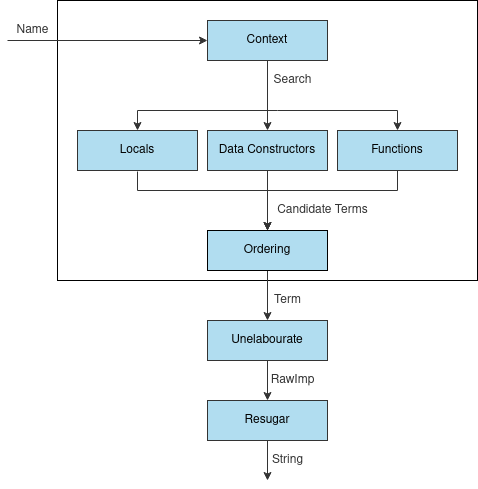
\includegraphics[scale=0.55]{./Resource/syn.png}
\captionof{figure}{Synthesising Terms}
\end{Figure}

\begin{Figure}
\centering
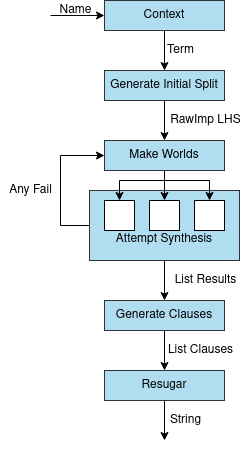
\includegraphics[scale=0.6]{./Resource/worlds.png}
\captionof{figure}{Synthesising Definitions}
\end{Figure}
\end{multicols}


\subsection{Extensions to the language}
\label{sec:org92a89c9}
The language has been extended with user inserted holes of the form \texttt{?hole\_name}. 
A constructor \texttt{IHole : Name -> RawImp} has been added to the RawImp 
data type and the parser extended to accept the new syntax. The 
unification state has also been extended with a sorted map of Names
to user holes, when IHoles are encountered during processing they are 
added to the map. The \texttt{Def} type was extended with a 
\texttt{MetaVar : (vars : List Name) -> Env Term vars -> (retTy : Term vars) -> Def}, 
\texttt{MetaVar} stores the local environment in which the metavariable is 
defined, along with it's return type, and the names in scope.
User provided holes should only appear on the right hand side of 
pattern matching definitions, thus there should always exist an expected 
type whenever an \texttt{IHole} is elaborated, during elaboration of holes, we get
the expected term, and use it to generate a new \texttt{Meta} term, with a
\texttt{MetaVar} definition using the environment and expected term.

To improve performance, certain other information has been added to the unification state, two sorted maps of names, one to functions and one to types
with the purpose of reducing the number of terms enumerated by the synthesiser as the 
context contains metavariables created during unification, causing it to quickly blow up in size  with values which could not lead to 
a candidate term. 
The processing of definitions has been extended to add new types and functions to these maps. Functions are added 
after the type is processed, allowing them to be used during synthesis, without having been implemented. 

The unification of TinyIdris fails with an error when a term is ill typed, 
in regular use this is the desired outcome, however when synthesising 
terms, the unification being performed is unsafe, since it list almost
guaranteed to be used on terms which will not unify, thus it has been 
extended to handle failure. The unification algorithm was also extended
to support the unification of binders, which is necessary when 
synthesising binders.  

Synthesis also create the need for new error messages, as certain exceptions
may occur that did not before, such as the name being provided not being found in the context, 
or having an invalid definition.
\subsection{Synthesising Individual Terms}
\label{sec:orgc850bb8}

A \texttt{Search} is represented internally as: 
\begin{itemize}
\item A \texttt{Nat} depth
\item The \texttt{Name} for the expression being synthesised.
\item The \texttt{Env} Local environment.
\item The \texttt{RawImp} left hand side of the target term.
\item A \texttt{Term vars} target type.
\end{itemize}

The depth is introduced to avoid termination issues. When synthesising a term of type \texttt{Nat}, the depth first nature of the 
search would lead to termination issues without a specified depth, for example when synthesising a \texttt{Nat}, it would attempt 
the \texttt{Suc} constructor, which takes a \texttt{Nat} argument, and so on. An initial depth of 4 has been found to be sufficiently deep 
to provide useful results, and not hinder performance. 

The name, environment and target type play an active role in synthesis, while the left hand side is used to check the term 
synthesised is structurally different from that on the left hand side. 

\begin{center}
\begin{minted}[obeytabs=true,tabsize=2]{idris}
record Search (vars : List Name) where
 constructor MkSearch
 depth : Nat
 name : Name
 env : Env Term vars
 lhs : RawImp
 target : Term vars 

synthesise : {vars : _} -> 
			 {auto c : Ref Ctxt Defs} -> 
			 {auto u : Ref UST UState} ->
			 Search vars -> Core (List (Term vars))

\end{minted}
\end{center}


Not all terms may be synthesised, we are only able to construct terms with a type as a type. The algorithm begins by 
inspecting the target type. If the type is a pi binder then we may construct a lambda with  
the argument type, and attempting to synthesise the scope.

If the type is of type \texttt{Type} then we are able to synthesise valid terms by using anything of type Type in the context,
however, this will lead to several incorrect answers being generated. Since types are passed in explicitly as patterns, 
we restrict the usable types to only those that have been passed in, since generally these will be the desired ones, 
as they frequently occur while synthesising arguments to candidate terms, since every argument must be explicitly passed.

After moving through each pi binder, the resulting scope must be an application of a type constructor to zero or more
arguments. If this is not the case, or the maximum depth has been reached, then the algorithm will check the local 
variables in scope for a term of the given type, which will only require a maximum of two passes of the environment,
before terminating. 

If the term is a valid application or type constructor then synthesis is attempted first by checking the 
local variables and then trying type constructors, followed by function definitions. When synthesising a term, a list of potential 
candidates will be returned, which may then be ordered based on some heuristic.

\subsubsection{Searching Locals}
\label{sec:orgbc2d082}
The algorithm first attempts to check the local environment for valid terms, this is mostly common when defining the 
base case of a recursive function, or when synthesising arguments for an top level term being synthesised. The process is split 
into two stages. 

Since only PVar and Lam binders result in a usable term being brought into scope the first stage consists of traversing
the environment and filtering out all of the un-usable binders, if a term is valid then we must construct a \texttt{Local} 
term referencing the name, the list of usable local variables is then passed to the second stage, which traverses the 
list and gets the binder from the environment. Unification is attempted between the target and the type of the binder,
if no constraints are generated then the Local term is accepted, and the rest of the environment is checked. 

If the binder unification fails, and the depth is non-zero, then a the type of the binder is checked, if it is a 
function type then the arguments are filled by metavariables and unification is once again attempted, if this 
succeeds then terms for each of the functions arguments are searched for, if successful an application is returned. This
is necessary for higher order functions to be synthesised.   

\subsubsection{Searching Globals}
\label{sec:org8039f5d}

Synthesis via data constructors and function definitions
both follow the same process. Data constructors are attempted
first, under the assumption that this will be the more likely solution.
However this may be overridden by any ordering heuristic used.

\begin{center}
\begin{minted}[obeytabs=true,tabsize=2]{idris}
tryDef : {vars : _} ->
		 {auto c : Ref Ctxt Defs} -> 
		 {auto u : Ref UST UState} ->
		 Search vars -> Name -> NameType ->
		 Term [] -> Core (List (Term vars))

tryIfSuccessful : {vars :_} ->
				  {auto c : Ref Ctxt Defs} ->
				  {auto u : Ref UST UState} ->
				  (Search vars) ->
				  Name -> NameType ->
				  NF vars -> Core (List (Term vars))
\end{minted}
\end{center}

When attempting to use a global definition, the problem is represented as a
name, nametype and closed term for the type of the definition. 
Each type will be of the form \texttt{p\textsubscript{1} -> ... -> p\textsubscript{n} -> r} where p\textsubscript{1} \ldots{} p\textsubscript{n} are 
arguments to the function and r is an application of a type constructor
to zero or more arguments. To avoid synthesising definitions which 
will result in an invalid term, metavariables are constructed for each binder and 
unification is attempted between the resulting type and the target type. If 
successful, a depth first traversal of the arguments takes place, synthesising terms for 
each, otherwise the search is stopped, and the algorithm
moves on to the next definition to be attempted. 

When synthesising arguments, it is possible that arguments deeper into the binder
may depend on arguments that have been previously passed in, therefore branching 
occurs as we move down through the binder. For each branch, the scope of the binder
is normalised using the synthesised term to construct a closure and unification is 
attempted between the scope and the target in the same fashion outlined above, 
if this fails then the branch is killed, otherwise the process is repeated for the 
scope. If the term passed in is not a Pi binder then we have reached the end of the 
arguments, and a Reference to the type constructor is returned, to which the 
synthesised terms may be applied. 

\subsubsection{Structural Recursion Checking}
\label{sec:orgb4d20b2}
The structural recursion check is conservative, in that it does not reduce terms, 
so may deny terms which are in fact structurally different. It checks that each name
present in the right hand side term is present in the left hand side term, if the right 
hand side is a binder then it is assumed not to be different. The check has been designed
this way to avoid terms being allowed because their arguments are different, however they 
are simply in a different order.  	

\subsection{Synthesising Definitions}
\label{sec:org7318356}

The problem of synthesising definitions utilises the synthesiser for
terms, however has the added complexity of introducing pattern matching, 
and combining the resulting terms. 

The only information available initially is the type 
signature of the function, from that, an initial left hand side RawImp
term that has no case splits is constructed. As a heuristic no synthesis 
is attempted at this stage, as typically functions are longer than a single 
case, and this could lead to valid, however incorrect definitions being
synthesised, any term which may be correctly synthesised at this stage will 
also be correct after splitting the cases, thus the negatives of this decision
are outweighed by the positives.

\subsubsection{Pattern Matching}
\label{sec:org38930cc}
The splitting algorithm receives either a singleton list containing the initial
left hand side, or a list of multiple which have been generated by a previous split, 
each of which is split again. Each lhs at the beginning will have
at least one unique term, which will not be split on, so every generated
left hand side will be unique. Any invalid terms generated are filtered out by 
the type checker. 

The terms split on will be the leftmost type constructor. Following a strict 
left to right split will lead to multiple redundant splits, this problem is 
exacerbated since each argument must be passed explicitly. To reduce this, 
a traversal of the generated split occurs, which uses the type information 
available from the initial split to fill in any implicit arguments generated, 
and if the new information provided by the split results in any deeper terms 
being forced into a certain pattern. Again the resulting left hand sides are
checked by the type checker to ensure their correctness, the traversal repeats for
each new split generated. Each lhs is split
into its own world, for which synthesis is attempted. If each world results 
in a valid term, then combining the worlds into a definition is attempted, if this
results in a valid definition, it is accepted, otherwise each world is further
split, a potential future optimisation could be to only split the worlds that are 
unsuccessful.

For each world to be synthesised the RawImp left hand side must be 
converted into an environment and a term, a list of candidates may then be 
synthesised for the target term. Synthesis is attempted for each remaining world, 
if any fail then the process is killed, returning to the splitting stage, otherwise the top term synthesised
is taken to avoid a blow up in defs being synthesised. The selected term is
converted into a clause, which is returned with each of the other clauses synthesised. 

\subsubsection{Combining Clauses}
\label{sec:org909acde}
TinyIdris has a built in CaseTree representation for clauses, when the synthesiser
returns a set of clauses, it is combined using this, ensuring the correctness
of the definition. Each definition is then returned, along with the list of clauses
to be converted into source code for the user.

TinyIdris does not have any termination checking built, therefore care
must be taken to ensure that where a recursive definition is synthesised,
a check is in place to ensure there is a base case, and that the function
will not recurse infinitely. 

After a valid term has been synthesised, be it a list of clauses or a valid term or 
full definition, this is converted back into a string in TinyIdris syntax for
the user to insert into the source file. 

\begin{center}
\begin{figure}[htbp]
\centering
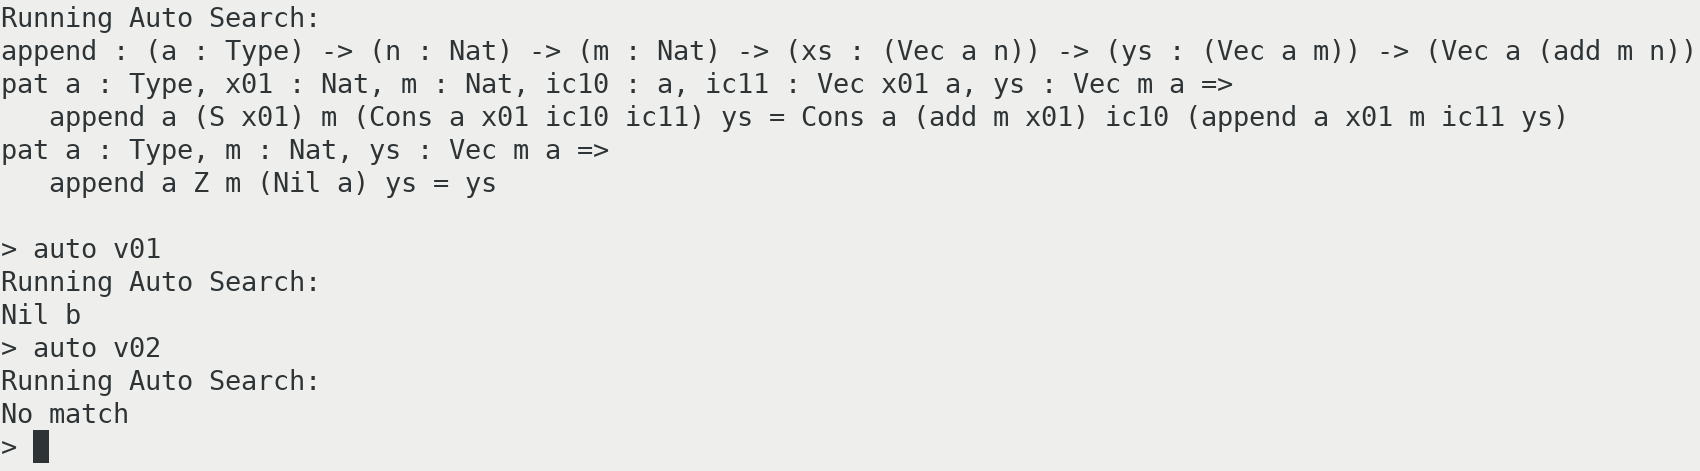
\includegraphics[scale=0.25]{./Resource/running.png}
\caption{Synthesising a definition, term, and failing on a term.}
\end{figure}
\end{center}

\clearpage

\section{Testing}
\label{sec:orgfd7bf85}

\subsection{Test Suite}

Testing takes the form of running the tool on various
function type signatures and evaluating the correctness
of the resulting definition if successful. The result
will be considered correct if on every possible input, it
will return the correct output. 

The test suite has been split into multiple categories, 
each testing a specific purpose. Each individual test 
has been selected from the test suite used to evaluate 
Agsy or that used to evaluate the tool Synquid.


\begin{itemize}
\item Lists
\item Vectors
\item Vectors with proofs
\item Equalities
\end{itemize}

The test suite has been designed to test the tool with varying
amounts of type information. As the level of type information
increases, the number of possible incorrect definitions decreases,
however the definitions themselves become more challenging for the
system to synthesise.

The list tests will be used to evaluate effectiveness of the
tools ability to synthesise terms without relying on detailed
type information. Vectors will contain the same examples as lists,
with the added type information of the length built in, it is expected that
this will reduce the number of trivial terms synthesised, without providing
detailed type information. Where the added type information present in
vectors is not enough for a successful attempt, more type information is added
to reduce the number of possible terms. Where applicable definitions will be
attempted, returning not only the result but a proof that the result satisfies
some property defining it' correctness. 

Testing Equalities focuses on the effectiveness of pattern matching
as the results will result from information from equality proofs provided
as arguments. 


\subsection{Testing Functionality}

The system provides two ways of testing the system on individual terms
where answers are present. 

Testing of individual holes can be carried out using the 
command \texttt{t} followed by the name of the hole. The system
will run the algorithm and test the results against an answer from
the answer file, the printout will return the hole name, expected result,
actual result and pass/fail. Alternatively holes can be synthesised in 
batches using the \texttt{test} command, which takes no arguments.
The system looks through the answer file, and for each name present,
attempts to synthesise a term, and returns the output detailed above,
the tool also returns a success rate over all the tests. 

\begin{center}
\begin{figure}[htbp]
\centering
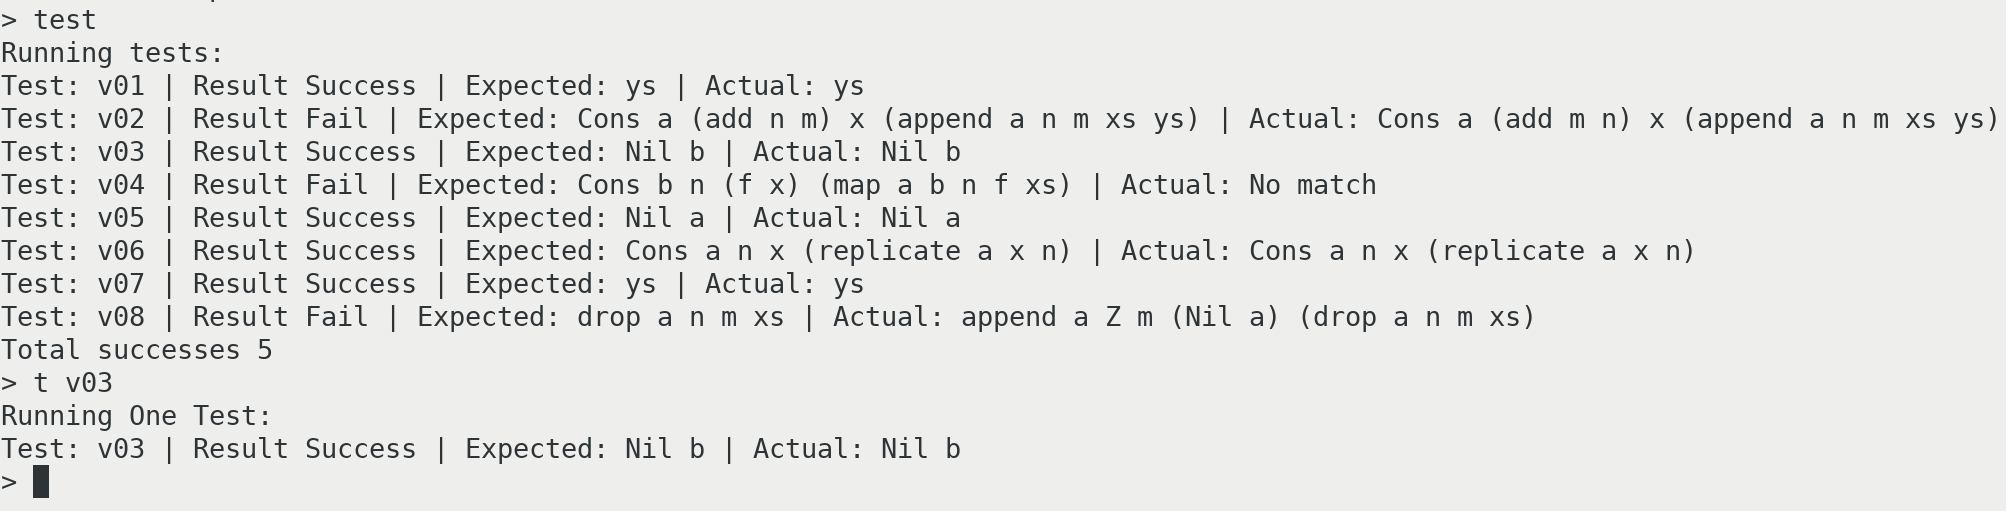
\includegraphics[scale=0.20]{./Resource/batch-test.png}
\caption{Batch and Individual Testing}
\end{figure}
\end{center}


\subsection{Testing Plan}

To test the tools, each has been converted into TinyIdris,
Idris, and Agda. To ensure that each tool has the same level
of information available to it, no tests use built in libraries,
instead opting to create exactly the same contexts for each.
Although many of the tests came from that the test suite used on
Synquid, the systems are different, and Synquid requires extra
information for synthesis, thus the results are not directly
comparable to the other systems.


Idris2 and TinyIdris both support generating
pattern matching definitions. Testing of these systems
were both attempted only on generating full definitions.
Neither Idris nor Agda support generating pattern matching
definitions, attempts were initially made before case splitting,
if both tools failed then the tests were repeated after
case splitting, the splits were done manually,
in the order most likely to present a result. This should not
provide any advantage to the two systems, since all valid splits
should be encountered by TinyIdris and Idris2.

\clearpage

\section{Evaluation}
\label{sec:org2fc5750}
\subsection{Initial Performance}
\label{sec:org9ac3710}

\subsubsection{Lists}
\label{sec:org840f301}
\begin{center}
\begin{tabular}{lllll}
Problem & TinyIdris & Idris & Idris2 & Agda\\
\hline
append & Fail & Fail & Pass & Fail\\
map & Fail & Fail & Pass & Fail\\
replicate & Fail & Fail & Pass & Fail\\
drop & Fail & Fail & Fail & Fail\\
foldr & Fail & Fail & Fail & Fail\\
is empty & Fail & Fail & Fail & Fail\\
is elem & Fail & Fail & Fail & Fail\\
duplicate & Fail & Fail & Fail & Fail\\
zip & Fail & Fail & Fail & Fail\\
i'th elem & Fail & Fail & Fail & Fail\\
index & Fail & Fail & Fail & Fail\\
\end{tabular}
\end{center}

\subsubsection{Vectors}
\label{sec:org20404d1}
\begin{center}
\begin{tabular}{lllll}
Problem & TinyIdris & Idris & Idris2 & Agda\\
\hline
append & Pass & Pass & Pass & Pass\\
map & Fail & Pass & Pass & Pass\\
replicate & Pass & Pass & Pass & Fail\\
drop & Fail & Fail & Pass & Fail\\
foldr & Fail & Fail & Fail & Fail\\
is empty & Fail & Fail & Fail & Fail\\
is elem & Fail & Fail & Fail & Fail\\
duplicate & Pass & Fail & Fail & Fail\\
zip & Fail & Pass & Pass & Fail\\
i'th elem & Fail & Fail & Fail & Fail\\
index & Fail & Fail & Fail & Fail\\
\end{tabular}
\end{center}

\subsubsection{Vectors With Proofs}
\label{sec:orge605b92}
\begin{center}
\begin{tabular}{lllll}
Problem & TinyIdris & Idris & Idris2 & Agda\\
\hline
is empty & Pass & Fail & Pass & Fail\\
is elem & Fail & Fail & Fail & Fail\\
duplicate & Fail & Fail & Pass & Fail\\
zip & Fail & Fail & Pass & Fail\\
i'th elem & Fail & Fail & Fail & Fail\\
index & Fail & Fail & Fail & Fail\\
\end{tabular}
\end{center}

\subsubsection{Equalities}
\label{sec:org3daf245}

\begin{center}
\begin{tabular}{lllll}
Problem & TinyIdris & Idris & Idris2 & Agda\\
\hline
plus commutes & Fail & Fail & Fail & Fail\\
plus Suc & Fail & Fail & Fail & Fail\\
symmetry & Fail & Pass & Pass & Fail\\
transitivity & Fail & Pass & Pass & Pass\\
congruence & Fail & Pass & Pass & Pass\\
list(vec(list)) = list & Fail & Pass & Pass & Pass\\
vec(list(list)) = vec & Fail & Fail & Pass & Fail\\
disjoint union apply & Fail & Fail & Fail & Fail\\
a = not not a & Fail & Fail & Fail & Fail\\
not not not a = not a & Fail & Fail & Pass & Fail\\
\end{tabular}
\end{center}

\subsection{Evaluation of performance}
\label{sec:org4c9aa94}
The overall performance of the system while testing 
the lists was poor, unable to synthesise any of the 
test cases, this was the expected outcome, since
there is a lack of type information to adequately cut out 
many of the incorrect results, with no results being correctly 
synthesised. 

With the added information available with vectors the tool was 
able to perform better, correctly synthesising 3 of the test cases,
somewhat surprisingly, it was unable to synthesise certain functions
such as 'map', which seems not unlike other examples that it was able 
to synthesise. Certain failed results from the vector test set result
from the the ordering heuristic, which does not take into account the
likelihood of recursion, and that the heuristic may be different
when synthesising arguments for terms and synthesising the top level
term itself.

Further inspection of the tools output confirms that indeed, for some
functions, such as \textit{drop}, the correct definition was
synthesised, however the ordering heuristic did not place it in the
top place. 

When provided with extra  type information the algorithm performed
worse, unable to synthesise terms that previously it was able to.
In certain cases it is clear that when provided with a possibility
that can be trivially constructed, then this will be the favoured
result. Again, this may be a result of the ordering heuristic.
While the extra type information reduces the number of correct 
synthesisable terms, it also increases the difficulty of the 
searches, increasing the number of constraints that must be satisfied. 

In the event that the tool ran for longer than 1 minute, the
test was stopped, and the result considered a fail. In many of
the types that may be generated by way of many different
functions, the tool required longer than this time limit, this suggests
that a depth alone is not sufficient, with the tool timing out after
a certain time limit, returning any results that have been successfully
generated. 

TinyIdris uses normalisation by evaluation, this, combined with the
explicitness of all arguments, impacts the results
produced by the tool. In certain cases, it was able to synthesise
unexpected, however correct results, for example when synthesising a
\texttt{Vect (add n m) a}, the tool passed \texttt{add m n} as the
length. This displays the tool is able to see relationships, making
some of the failed results surprising.

\subsection{Comparison to other systems}
\label{sec:orga2f8b7e}
The results, when compared to the two older systems, Idris and Agda, 
performed comparably, with the exception of the Equalities tests,
where both clearly outperformed the tool. The tests used self defined
data types, to remove any advantage the other systems would have by
accessing any information available in the libraries. This may go some
way towards explaining the relatively poor performance of Agsy during
the Equalities section, as it relies on built in tactics.
The Equalities test were designed to test the
tools ability to gain new information via case splitting, the failure
suggests that the tool is either unable to effectively generate new
information, or is not effectively utilising it. This may result from
the less sophisticated type system present in the TinyIdris language.

In other test suites, Idris and Agsy were able to synthesise terms,
such as map, that the TinyIdris tool was not able to, this suggests
that the tool is unable to cope with the added complexity of using
higher order functions, this could result from the depth cutting off
the search, or suggests a deficiency in the way the tool synthesises
function application.

The tool was outperformed in each section by the Idris2 system,
given the similarities within the systems this suggests that the
ordering heuristic used in the Idris2 system is superior, and that
recursive functions should be prioritised over using any function
from the context.

The test cases used in the first three sections came from the testing
used in the Synquid system, the although the languages and type systems
are not comparable, the overwhelming difference in performance between
Synquid and each of the systems tests suggests that the use of
refinement types and an SMT solver is superior than using dependent
types for synthesis. Definitions in Synquid can be verbose, with
certain information required for successful synthesis. This problem is
present within the TinyIdris system also, as specifying complex
properties often becomes cumbersome, and can be vastly more difficult
than defining the functions themselves. While this has benefits for
program correctness, it limits the usefulness of any program synthesis
functionality. Unlike Synquid, the TinyIdris language has no concept of
case splitting outside of pattern matching,
meaning the system is unable to operate differently based on the result
of any recursive calls or function applications. This severely limits
the effectiveness of synthesis to mostly synthesising trivial cases,
that have no element of choice. While the other systems have it
available it is not used, this suggests that encoding the idea of
choice into any synthesis tool may lead to greatly improved success
rates.


\subsection{Conclusions}
It is clear that further experimentation with the results of the
tool is required, in order to fully understand what caused the poor
results, including experimentation with different ordering heuristics,
attempting to synthesise multiple pattern matching definitions and
attempting to find out if the inferior type system found in TinyIdris
may have an affect on the results. The tool could be improved through
extending the language with more features, additionally,
experimentation should be carried out on a more fully featured system.
Implementing synthesis using any function that results in a valid type
proved not to be a fruitful approach, however, synthesis using
global function definitions, and attempting case splits could lead to
improvements in the presence of built in heuristics guiding the
algorithm to choose sensible functions to attempt.
\nocite{*}
\bibliography{Report}  
\clearpage

\label{sec:org30d868f}
\section{Appendix A - Detailed Implementation}
\label{sec:org4318281}

\subsection{Synthesis}
Searches within the system are defined as a record type:

\begin{center}
  \begin{minted}{idris}
record Search (vars : List Name) where
 constructor MkSearch
 depth : Nat
 name : Name
 env : Env Term vars
 lhs : RawImp
 target : Term vars 
  \end{minted}
\end{center}

While this is not necessary for the functionality, it serves
to clean up the type signatures of functions, improving readability. 
The majority of the functionality is wrapped up in the \texttt{Core}
monad, which is a major part of the TinyIdris system, the Monad
is a wrapper around the IO Monad, which allows IO operations to be
carried out, \texttt{Core} extends this functionality to include
global references for the context and unification state. Since these
is required frequently, much of the functionality must occur inside
Core. 

When a search begins, the \texttt{run} function is called, this
has the purpose of checking which kind of search is being attempted by
checking the definition from the context, running the search, and
converting the result back into a string via the re-sugaring
functionality. In the event that the search is an individual term,
the results are filtered here to ensure that they are structurally
different from the left hand side.

\subsubsection{Individual Terms}
If the definition of the name being searched is a \texttt{MetaVar},
the left hand side of the clause it is defined in is retrieved from
the user holes map within the unification state, together with the
environment and return type from the \texttt{Def}, and the name,
this is combined to generate a search, on which the synthesise function
is called.

\begin{center}
  \begin{minted}{idris}
    synthesise : {vars : _} -> 
             {auto c : Ref Ctxt Defs} -> 
             {auto u : Ref UST UState} ->
             Search vars -> Core (List (Term vars))
  \end{minted}
\end{center}

The synthesis function when given a search will return a list of
candidate terms. The function operates by matching on the return
type, if it is a pi binder then the function is called recursively
with an extended environment taking in a lambda, and the scope. If the
target is of type \texttt{Type}, or the depth is zero then it searches the environment,
otherwise it performs a full search.

A full search is performed by trying local variables, then data constructors,
and finally function definitions. 

When searching definitions, we must be able to construct \texttt{Local} terms
referencing them, to do this the environment must be `re scoped'.

\begin{center}
  \begin{minted}{idris}
getUsableEnv : {vars : _} -> 
               (ns : List Name) ->
               Env Term vars ->
               List (Term (ns ++ vars))
getUsableEnv {vars = v :: vars} ns ((PVar x z) :: env) 
= let rest = getUsableEnv {vars = vars} (ns ++ [v]) env 
      MkVar var = weakenNS ns (MkVar First) in 
  Local _ var :: rewrite appendAssociative ns [v] vars in rest
  \end{minted}
\end{center}

Rescoping the environment consists of checking which terms from the 
environment are in a usable form, either lambdas or pattern variables.
The binder type is then weakened using a list of names that are passed in,
weakening is simply extending the list of names that are in scope for
a given term, a local referencing the original term is returned. A
proof of associativity is required to satisfy the type checker that
the list of names from the recursive call is correct. By calling
the \texttt{getUsableEnv} function with the empty list of names, the returned
terms will be in the scope \texttt{[] ++ vars} which is equal to
\texttt{vars}, the original scope.

Searching these terms consists of looking up the binder within the
environment, and attempting to unify its type with the return type.
If this is successful the local is returned, and the search continues
with the rest, if this is unsuccessful, and the depth is greater than
0 then the type of the binder is checked in case it is a function with
the correct return type. If it is then synthesis is attempted for the arguments,
otherwise the search continues with the rest of the locals.

In order to check if the result of a pi binder is the type we are
looking for, the binder must be normalised, which can then be filled
with metavariables, and quoted back to a term. Unification can then be
attempted between the return type and the filled type, which will
either succeed, with the constraints that metavariables are equal to
certain types, or fail.

\begin{center}
  \begin{minted}{idris}
fillMetas : {vars : _} -> 
            {auto c : Ref Ctxt Defs} ->
            {auto u : Ref UST UState} ->
            Env Term vars -> NF vars ->
            Core (NF vars , List (Term vars, Name))
fillMetas env (NBind n (Pi n' pinfo tm) scope) 
  = do defs <- get Ctxt 
       nm <- genName "filling"
       mta <- newMeta env nm !(quote defs env tm) Hole
       (f , args) <- fillMetas env !(scope defs (toClosure env mta))
       pure (f , (mta , nm) :: args)
fillMetas env tm = pure (tm , [])
  \end{minted}
\end{center}

The task of filling terms with metavariables is carried out by the
\texttt{fillMetas} function, which takes an environment and a value scoped
by this environment. A metavariable for the argument type is generated
and added to the context, the term is converted to a closure and passed
into the scope, with which a recursive call is made to return the
term at the end of the scope. A list of the metavariables along with
their names are returned for deletion later, to avoid cluttering the
context.

The process for synthesising local functions follows the
same process as for constructors, and function definitions. The process
outlined above is handled for them by the tryDef function. The
synthesis function determines the correct data constructors for the
given type, and accesses the functions from the unification state,
for each it calls the \texttt{tryDef} function, and concatenates the results.

The process for synthesising arguments is similar, and is handled via
the \texttt{tryIfScucessful} function.

\begin{center}
  \begin{minted}{idris}
tryIfSuccessful : {vars :_} ->
                  {auto c : Ref Ctxt Defs} ->
                  {auto u : Ref UST UState} ->
                  (Search vars) ->
                  Name -> NameType ->
                  NF vars -> Core (List (Term vars))
tryIfSuccessful s@(MkSearch (S depth) name env lhs target) n nty (NBind m (Pi nm pinfo tm) sc)
  = do defs <- get Ctxt
       (tm' :: ts) <- synthesise (MkSearch (pred depth) m env lhs !(quote defs env tm))
        | _ => none
       results <- traverse help (tm' :: ts)
       pure $ concat results
  where help : Term vars ->
               Core (List (Term vars))
        help tm
         = do defs <- get Ctxt
              sc' <- sc defs (toClosure env tm)
              (filled , fas) <- fillMetas env sc'
              Just ures <- tryUnify env target !(quote defs env filled)
               | _ => none 
              (r :: rs) <- tryIfSuccessful s n nty sc'
               | _ => none
              pure $ map (\ z => App z tm) (r :: rs)
tryIfSuccessful (MkSearch 0 name env lhs target) n nty tm = none
tryIfSuccessful (MkSearch depth name env lhs target) n nty tm 
  = do defs <- get Ctxt
       Just (MkUnifyResult [] holesSolved) <- tryUnify env target !(quote defs env tm)
        | _ => none  
       pure [Ref nty n]
  \end{minted}
\end{center}
       
When synthesising arguments, the function must handle 
branching of each term synthesised, killing branches when synthesis is unsuccessful.
The function operates by synthesising a term for the argument, when
this takes place the depth is reduced to ensure termination of the
program. A new branch is created for each of the synthesised terms.
Each branch is carried out by the helper function, which attempts unification,
and continues down the branch if successful. This branching is required
as each scope may depend on the argument synthesised, therefore it must be passed
as a closure into the value. When every argument has been synthesised,
a reference to the constructor or function is returned, to which the
synthesised arguments are applied.

\subsubsection{Pattern Matching Definitions}

The generation of pattern matching definitions can be split into three main
problems, splitting the left hand side, handling synthesis of multiple
cases, and combining cases. All of which is handled by the
\texttt{defSearch} function.

\begin{center}
  \begin{minted}{idris}
defSearch : {auto c : Ref Ctxt Defs} ->
        {auto u : Ref UST UState} -> 
        GlobalDef -> Name -> List RawImp -> Nat ->
        Core (Maybe (Def, List (Clause, RawImp, RawImp)))
defSearch def n lhs splits = 
  do cs@(c :: cases) <- traverse (splitLhs False splits) lhs | _ => pure Nothing
     gs@(p :: ps) <- filterCheckable (concat cs) | _ => pure Nothing
     let gs' = concat !(traverse (splitSingles (S splits)) (map (\ (_,_,a) => a) gs)) 
     gs''@(p' :: ps') <- filterCheckable (map (\ g => (g,())) gs') | _ => nothing
     Just res <- synthesisePM n (type def)
                  !(traverse (\ (_,gd,ri,_) => pure $ getSearchData !(getTerm gd) [] ri) gs'')
      | _ => defSearch def n (map (\ (_,_,ri,_) => ri) gs'') (S splits) 
     pure $ Just res
  \end{minted}
\end{center}

The tool, when given a single left hand side, performs a split
initially, this is a heuristic to help prevent against correct,
but undesirable terms. For certain types, for example, \texttt{Maybe},
the tool will always be able to synthesise trivially true terms, \texttt{Nothing}, for \texttt{Maybe}, which
is unlikely to be the desired solution for each case.

To ensure that synthesis is only performed on
correct terms, any invalid terms generated are filtered out by the type checker.
This approach leads to redundant splits, therefore, each argument that depends
on the split argument is checked in case it has been forced into being constructed only
one way, if it has, then it is also split, this helps to reduce the number of
cases generated. For example, an initial split on \texttt{n : Nat} being split to Z, the \texttt{Cons}
constructor will no longer apply for any vectors of length n, thus the vector
split to Nil would be accepted.

If a set of splits has been generated, the synthesis is attempted, otherwise the
algorithm fails. Generating splits will be covered in more detail in the next section.

When attempting synthesis on a set of left hand sides, each is split into its own
world. If synthesis for each world is successful then it is checked that at least
one does not contain a recursive call, this is required since TinyIdris features no termination
checking, however this check is not strong enough to prevent circular definitions occurring from
mutually recursive functions. If the check passes, the clauses are combined into a definition
by constructing a case tree, which is returned along side the clauses to be converted back
into a string. 

\begin{center}
  \begin{minted}{idris}
synthesiseWorlds : {auto c : Ref Ctxt Defs} -> 
                   {auto u : Ref UST UState} -> 
                   Name ->
                   List (vars ** (Env Term vars , Term vars, RawImp)) ->
                   Core (Maybe (List (Clause, RawImp, RawImp)))
synthesiseWorlds n [] = pure $ Just []
synthesiseWorlds n ((vars ** (env, tm, ri)) :: xs)
 = do let s = (MkSearch 4 n env ri tm)
      (t :: ts) <- synthesise s | _ => nothing  
      (t' :: ts') <- filterM (structuralRecursionCheck env ri) (t :: ts) | _ => nothing
      Just rest <- synthesiseWorlds n xs | _ => nothing
      clause <- getClause (s, t', ri)
      pure $ Just (clause :: rest)
  \end{minted}
\end{center}

The algorithm recursively loops through each world attempting to synthesise a term of
the correct return type. If any fail the process is stopped. The first term is taken,
to avoid greatly increasing the number of cases synthesis is being attempted for. If
each world is able to be synthesised, the resulting information is combined to a
clause, which is returned along with the rest of the clauses. Generating each clause
is straightforward, checking the left hand side, and un-elabourating the right hand side.

\subsubsection{Pattern matching}

Pattern matching occurs in two forms, when generating a split given a
left hand side, and refining a left hand side which has been split,
and contains arguments that depend on the split argument.

It is only type constructors that may be split on currently,
however a potential extension could look to split type constructors
that have been applied to data constructors on the left hand side.

The initial case simply traverses the term left to right,
looking for the first argument which may be split.
For each of the data constructors constructing the argument type,
patterns are generated taking in their required arguments, and
every reference to the argument within the scope is replaced with an
application of the data constructor to it's arguments.

To construct each pattern, a unique name is generated, which is
referenced using an \texttt{IVar} in the application, and an
\texttt{IPatvar} taking the name in is generated, with its type being
left implicit. The resulting patterns and scope can then be merged
with the rest of the left hand side. 

The second, and more complex case has two main functions, 
to check if any arguments in a RawImp term are forced into being
constructed only by a single constructor, and attempting to fill
in as many implicit arguments as possible. The process repeats
while there are names that depend on a previously split term that
have not been checked yet.

\begin{center}
  \begin{minted}{idris}
splitSingles : {auto c : Ref Ctxt Defs} -> 
               {auto u : Ref UST UState} ->
               Nat -> (RawImp, List Name) -> 
               Core (List RawImp)
splitSingles splits (tm,[]) = pure [tm]
splitSingles splits (tm,(n :: ns)) 
  = do upd <- splitSingle tm n 
       [(_,_,updated, newnames)] <- filterCheckable upd
         | _ => splitSingles splits (tm, ns)
       splitSingles (S splits) (updated, ns ++ newnames)
  where  
        splitSingle : RawImp -> Name -> Core (List (RawImp, List Name))
        splitSingle (IPatvar x ty scope) n
          = do defs <- get Ctxt
               (tm , gd) <- checkTerm [] (IPatvar x ty scope) Nothing
               norm <- nf defs [] tm
               Just (pats, app) <- getSplit splits norm n [] | _ => none
               let (Just pre, suf) = splitOnN (IPatvar x ty scope) n | _ => none
               let front = pre . pats 
                   (newsc, names) = fixUpScope n suf app
               newtm <- fillImplicits (front newsc) [] (front newsc) 
               pure [(newtm, names)] 
        splitSingle _ _ = none
  \end{minted}
\end{center}

For each of the names, the left hand side is checked and normalised,
this is to provide the algorithm with information about arguments to
the type constructors via closures stored within the normal form,
the \texttt{getSplit} function is called.

The \texttt{getSplit} function checks that the argument is a type
constructor with only one valid way of constructing it. It then
normalises and traverses the data constructors type, to reach
the return type, which should be the same as the original type.
The list of closures in both type constructor values are zipped
together, and a second traversal of the normal form occurs. The
purpose of this is to check if any of the arguments to the constructor
appear in the resulting type. If they do, no pattern variables
are required, and the constructor can be applied to the name from the
original closure, since it must have been passed in before this argument
was reached. If an argument is not present within the closure then
an implicit argument is taken in by a pattern variable, and applied to
the constructor. This results in a \texttt{RawImp} for the pattern variables
required, and the application. 

The initial \texttt{RawImp} term is split into two parts, the
patterns occurring before the name appears, and everything that
appears after the name. The parts are combined with the new patterns
and applications, generating the \texttt{RawImp} Term,
and a list of names that depend on the now split argument.

Before continuing this process with the rest of the names,
the algorithm attempts to use any information it has generated
to fill in any Implicit arguments, via the \texttt{fillImplicits} function.

\begin{center}
  \begin{minted}{idris}
fillImplicits : {vars :_} ->
                {auto c : Ref Ctxt Defs} -> 
                {auto u : Ref UST UState} ->
                RawImp -> Env Term vars -> RawImp -> 
                Core RawImp 
fillImplicits (IPatvar x Implicit scope) env ri
  = do (tm, gd) <- checkTerm env Implicit (Just gType)
       let env' : Env Term (x :: vars)
                = (Lam x Explicit tm :: env)
       fillImplicits scope env' ri
       
fillImplicits (IPatvar x ty scope) env ri
 = do (tm, gd) <- checkTerm env ty Nothing
      let env' : Env Term (x :: vars) 
               = (Lam x Explicit tm) :: env
      fillImplicits scope env' ri

fillImplicits (IApp f a) env ri
 = do (ftm, gfty) <- checkTerm env f Nothing
      fty <- getNF gfty
      defs <- get Ctxt
      ri' <- fillImplicits f env ri
      case fty of
       (NBind x (Pi _ _ ty) sc) => 
         do
           (atm, gaty) <- checkTerm env a
                           (Just (glueBack defs env ty))                    
           case a of 
            (IVar y) => pure $ replaceImplicitAt y !(getTerm gaty) ri'
            (IApp y z) => fillImplicits (IApp y z) env ri'
            _ => pure ri'
       t => throw (GenericMsg "Not a function type")
fillImplicits tm env ri = pure ri
  \end{minted}
\end{center}

The \texttt{fillMetas} function repeatedly accepts arguments,
checking their term and extending the environment with them.
When it reaches the application at the end. Then progressively
moves through the arguments left to right, at which point it
may have enough information to fill in the type of any implicit
arguments with their expected type, however, this is not always
the case, as it relied on the initial step of filling in implicits
via the closures to have resulted in a valid term.

\subsubsection{Un-Elabourating and Re-Sugaring}

The un-elabouration and re-sugaring algorithm are straightforward,
converting a \texttt{Term} back into \texttt{RawImp} and back \texttt{RawImp} to \texttt{String}.

When re-sugaring, the syntax of expressions will be dependent on it's location within a term,
thus certain conditional functions have been created to handle either case.
Re-Sugaring full definitions is split into re-sugaring the type
signature, followed by the list of clauses, which simply re-sugars the
left and right hand side of each, combining them, with an equals sign.
Re-Sugaring terms that appear on the left hand side in patterns
requires some extra care, since applications will be in the reverse
order from those on the right. 

\clearpage
\section{Appendix C - User Guide}

The system is built using the Idris2 programming language, due to
a lack of backwards comparability the required version is
\texttt{0.2.1} which can be located
\href{https://github.com/idris-lang/Idris2/tree/compat-0.2.1}{from the Idris2 GitHub}.

The installation of idris2 requires either chez scheme or racket,
details of how to install this can be found
\href{https://www.scheme.com/}{here}.

To install Idris2 the commands \texttt{make bootstrap SCHEME=chez}
then \texttt{make install} are run. Depending on the version of
scheme and operating system the first command may change to
\texttt{SCHEME=scheme} or \texttt{SCHEME=chezscheme}. 


The system can be accessed from \href{https://github.com/Ablach/tiny-idris-program-synthesis}{Github}. The tool is built using the command
\texttt{idris2 --install tinyidris.ipkg} while in the TinyIdris
directory. TinyIdris can be run using the \texttt{tinyidris}
executable located in the \texttt{build/exec} directory, and passing
the name of a '.tidr' test file. Test files are located within the \texttt{/Test/TestFiles} directory. If a new TinyIdris source file is created, then it
should be stored within the \texttt{Test/TestFiles}
directory, and an answer file of the same name created in the
\texttt{AnswerFiles} directory using the extension \texttt{.ans}.
The answer file may be left blank. 

While in the TinyIdris repl tree 4 commands may be issued. To evaluate
and type check an expression type the expression, with nothing before
it. To synthesise a definition or term, use the command \texttt{auto},
followed by the name of the hole or the function.
To test synthesis of an individual term run the command \texttt{t},
with the hole name as an argument, or to batch test a group of holes
within a file, simply run \texttt{test}, with no arguments.

In order for the last two commands to work the answer file must contain
solutions for the problem, any holes that do not habe a solution will
be skipped. Solutions are written in the answer file as
\texttt{<name> ! <solution>}.

To exit the tinyidris repl press Ctrl-C.

\end{document}
